%ju 28-Mai-22 FM_U08_Leistung_Mathebuch_Loesung.tex
\section{Leistung Übung 8
Mathebuch}\label{leistung-uebung-8-mathebuch}

Vgl. Mathebuch (\textcite{elbl:2016:technMa})

\textbf{S. 82 Aufgabe 4d}

\lstset{language=Python}% C, TeX, Bash, Python 
\begin{lstlisting}[
	%caption={}, label={code:}%% anpassen
][language=Python]
# geg:
I_ges = 0,35 A
U = 210 V
R_2 = 1000 Ohm = 1 k
# ges: I_1, I_2, R_ges, R_1, P_R_1, P_R_2
# Formel:
R_ges = U/I_ges
I_2 = U/R_2
I_ges = I_1 + I_2 -> I_1 = I_ges - I_2
R_1 = U/I_1
P_R_1 = U x I_1
P_R_2 = U x I_2
# Lösung:
R_ges = 600,0 Ohm
I_2 = 0,21 A
I_1 = 0,14 A
R_1 = 1500,0 Ohm
P_R_1 = 29,4 W
P_R_2 = 44,1 W
\end{lstlisting}

\textbf{S. 84 Aufgabe 4}

\lstset{language=Python}% C, TeX, Bash, Python 
\begin{lstlisting}[
	%caption={}, label={code:}%% anpassen
][language=Python]
# geg: Glühkerze
U_k = 10,5 V
P_k = 100 W
# ges: I_k, R_k
# Formel:
P = U x I -> I_k = P_k/U_k
R_k_1 = U_k/I_k (Var, 1)
P = U x I -> P = U^2/R
R_k_2 = (U_k x U_k)/P_k (Var, 2)
# Lösung:
I_k = 9,5238 A
R_k_1 = 1,1025 Ohm
R_k_2 = 1,1025 Ohm
\end{lstlisting}

\newpage

\textbf{S. 82 Aufgabe 3}

\begin{figure}[!ht]% hier: !ht
\centering
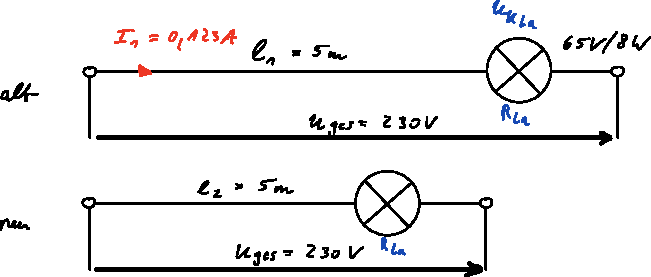
\includegraphics[width=0.6\textwidth]{images/Skizze/26_FM_Leistung_Mathebuch_A3.pdf}
\caption{FM Leistung Mathebuch A3}
%\label{fig:}%% anpassen
\end{figure}

\lstset{language=Python}% C, TeX, Bash, Python 
\begin{lstlisting}[
	%caption={}, label={code:}%% anpassen
][language=Python]
# geg: Leuchtstoffröhre 65V/8W Schaltung
U_ges = 230 V
U_k_La = 65 V
l_1 = 5 m
l_2 = 4 m
I_1 = 0,123 A = 123 mA
# ges: U_k_La_tat, P_La_tat
# Formel:
R_La = U_k_La/I_1
# R_l_1 = U_R_l_1/I_1
R_l_1 = (U_ges - U_k_La)/I_1
# Dreisatz
5 m = 1341,46 Ohm
4 m = x Ohm
R_l_2 = l_2 x R_l_1/l_1
R_ges_tat = R_l_2 + R_La
I_tat = U_ges/R_ges_tat
U_k_La_tat = R_La x I_tat
P_La_tat = U_k_La_tat x I_tat
# Lösung:
R_La = 528,4553 Ohm
R_l_1 = 1341,4634 Ohm
R_l_2 = 1073,1707 Ohm
R_ges_tat = 1601,626 Ohm
I_tat = 0,1436 A
U_k_La_tat = 75,8883 V
P_La_tat = 10,8979 W
\end{lstlisting}
